\titledquestion{Register allocation}
\droptotalpoints

You have to colour the following interference graph with three colours
(\verb+r1+, \verb+r2+, \verb+r3+ are precoulored):
\vspace{-1em}
\begin{center}
  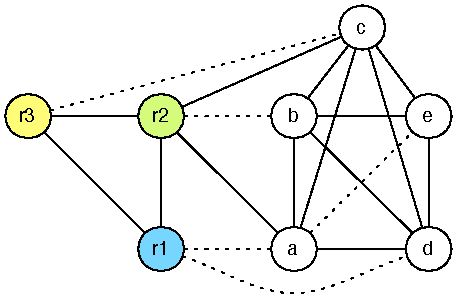
\includegraphics[scale=.85]{questions/register-allocation/interference-appel-11-3-1}
\end{center}

\begin{parts}
\part[5]
Should the next step be a \emph{spill}? Why (not)?

\begin{solution}
We cannot simplify, since all nodes are either precoloured or move-related.
But we can coalesce \Verb+a+ and \Verb+e+ (all neighbours of \Verb+e+
of significant degree are neighbors of \Verb+a+, George).
\end{solution}

\part[12]
Spill node \verb+c+ and continue the graph colouring until you can decide if this spill is an actual one.

\begin{solution}
We can coalesce \Verb+a+ and \Verb+e+, since the resulting node has no
neighbours of significant degree ($0<3$, Briggs).
For the same reason, we can coalesce \Verb+a e+ and \Verb+r1+ as well as
\Verb+b+ and \Verb+r3+.
We cannot coalesce \Verb+a e r1+ with \Verb+d+ since they interfere,
but we can simplify \Verb+d+.
Now we have only precoloured nodes and can bring back nodes, starting
with \Verb+d+.

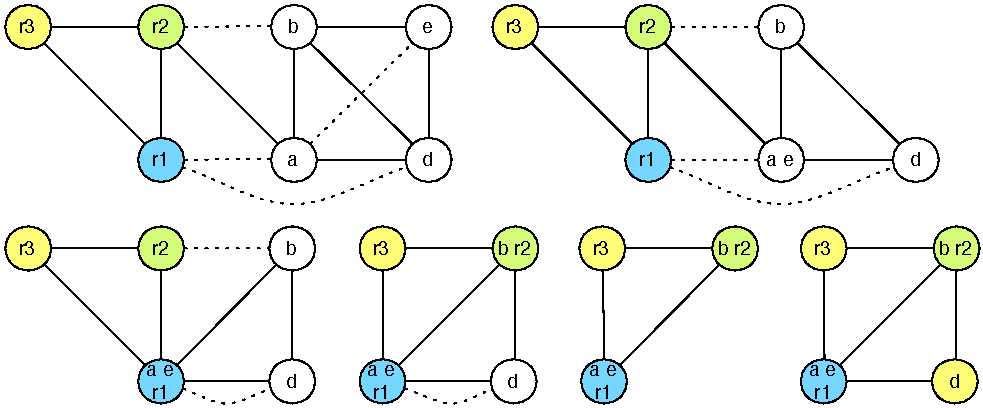
\includegraphics[scale=.85]{questions/register-allocation/colouring-appel-11-3-1}
\end{solution}

\part[1]
Is node \verb+c+ an actual spill?

\begin{solution}
Yes, since we cannot assign any colour to \Verb+c+.
\end{solution}

\part[2]
Perform the spill on the intermediate code from the previous question.

\begin{solution}
\begin{minipage}[t]{5cm}
\fvset{frame=lines}
\fvset{framesep=8pt}
\begin{Verbatim}
     c1 := r3
     M[cloc] := c1
     a := r1
     b := r2
     d := 0 
     e := a      
l1:  d := d + b
     e := e - 1
     if e > 0 goto l1
     r1 := d
     c2 := M[cloc]
     r3 := c2
     return     
\end{Verbatim}
\end{minipage}

\end{solution}

\end{parts}
 
